\documentclass{article}
\usepackage{ucs}
\usepackage[utf8x]{inputenc}
\usepackage{graphicx}
\title{Reducering af brændstofforbrug ved hastighedstilpasining til trafiklys}
\date{}
\begin{document}
\maketitle

Ved kendskab til trafiksignalerne kan den enkelte bil tilpasse sin hastighed således det næste kryds nåes i det øjeblik det skifter til grønt.
I mange tilfælde kan standsninger helt undgåes og man opnår et jævnt flow gennem trafiklysene.
Herved reduceres den dyre acceleration.
Simuleringer viser at brændstofforbruget kan mindskes med ca. 25 \% for den enkelte bilist uden nævneværdig negativ påvirkning af øvrig trafik i forhold til almindelig kørsel.
Besparelsen opnås allerede for den første bil og bevares ved opskalering.

Systemet fungerer bedst ved uden for myldretiden og med tidsstyret lyskryds, men kan også bruges i andre tilfælde, dog med et potentielt mindre udbytte for bilisterne.

Systemet implementeres på en smartphone, der konstant udregner den bedste hastighed og viser denne til bilisten. 
For at systemet kan fungere optimalt, kræver det adgang til aflæsning af trafiksignalernes tilstand og at bilisten angiver den rute han vil følge.
Der er derfor få invisteringsudgifter men høj udbytte for bilister.

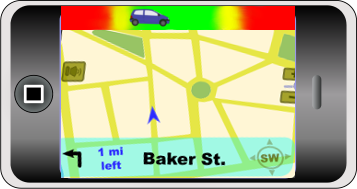
\includegraphics[width=1\textwidth]{images/product.png}


GreenSpeed
GreenFlow

\end{document}














